Expressions describing or referring to objects in visual scenes typically include object names: e.g.,  \emph{cheesecake} or  \emph{dessert}  in Figure~\ref{fig:ex1}.
Determining these object names is a core aspect of virtually every language \& vision task, ranging from e.g.\ referring expression generation to visual dialogue \cite{add-refs}.
We investigate the extent to which there is variation in the names chosen by different people for the same object, and its implications for research in language \& vision.
% For instance, the objects in Figure \ref{fig:cake} could be named \refexp{cake}, \refexp{cheesecake}, \refexp{dessert}, \refexp{sweet}, \refexp{pastry}, \refexp{food} etc.

\begin{figure}[htbp]
\begin{center}
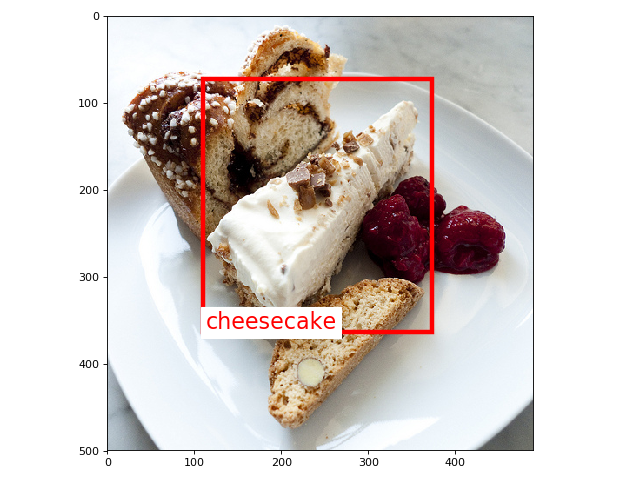
\includegraphics[height=3cm]{figures/cheesecake.png}
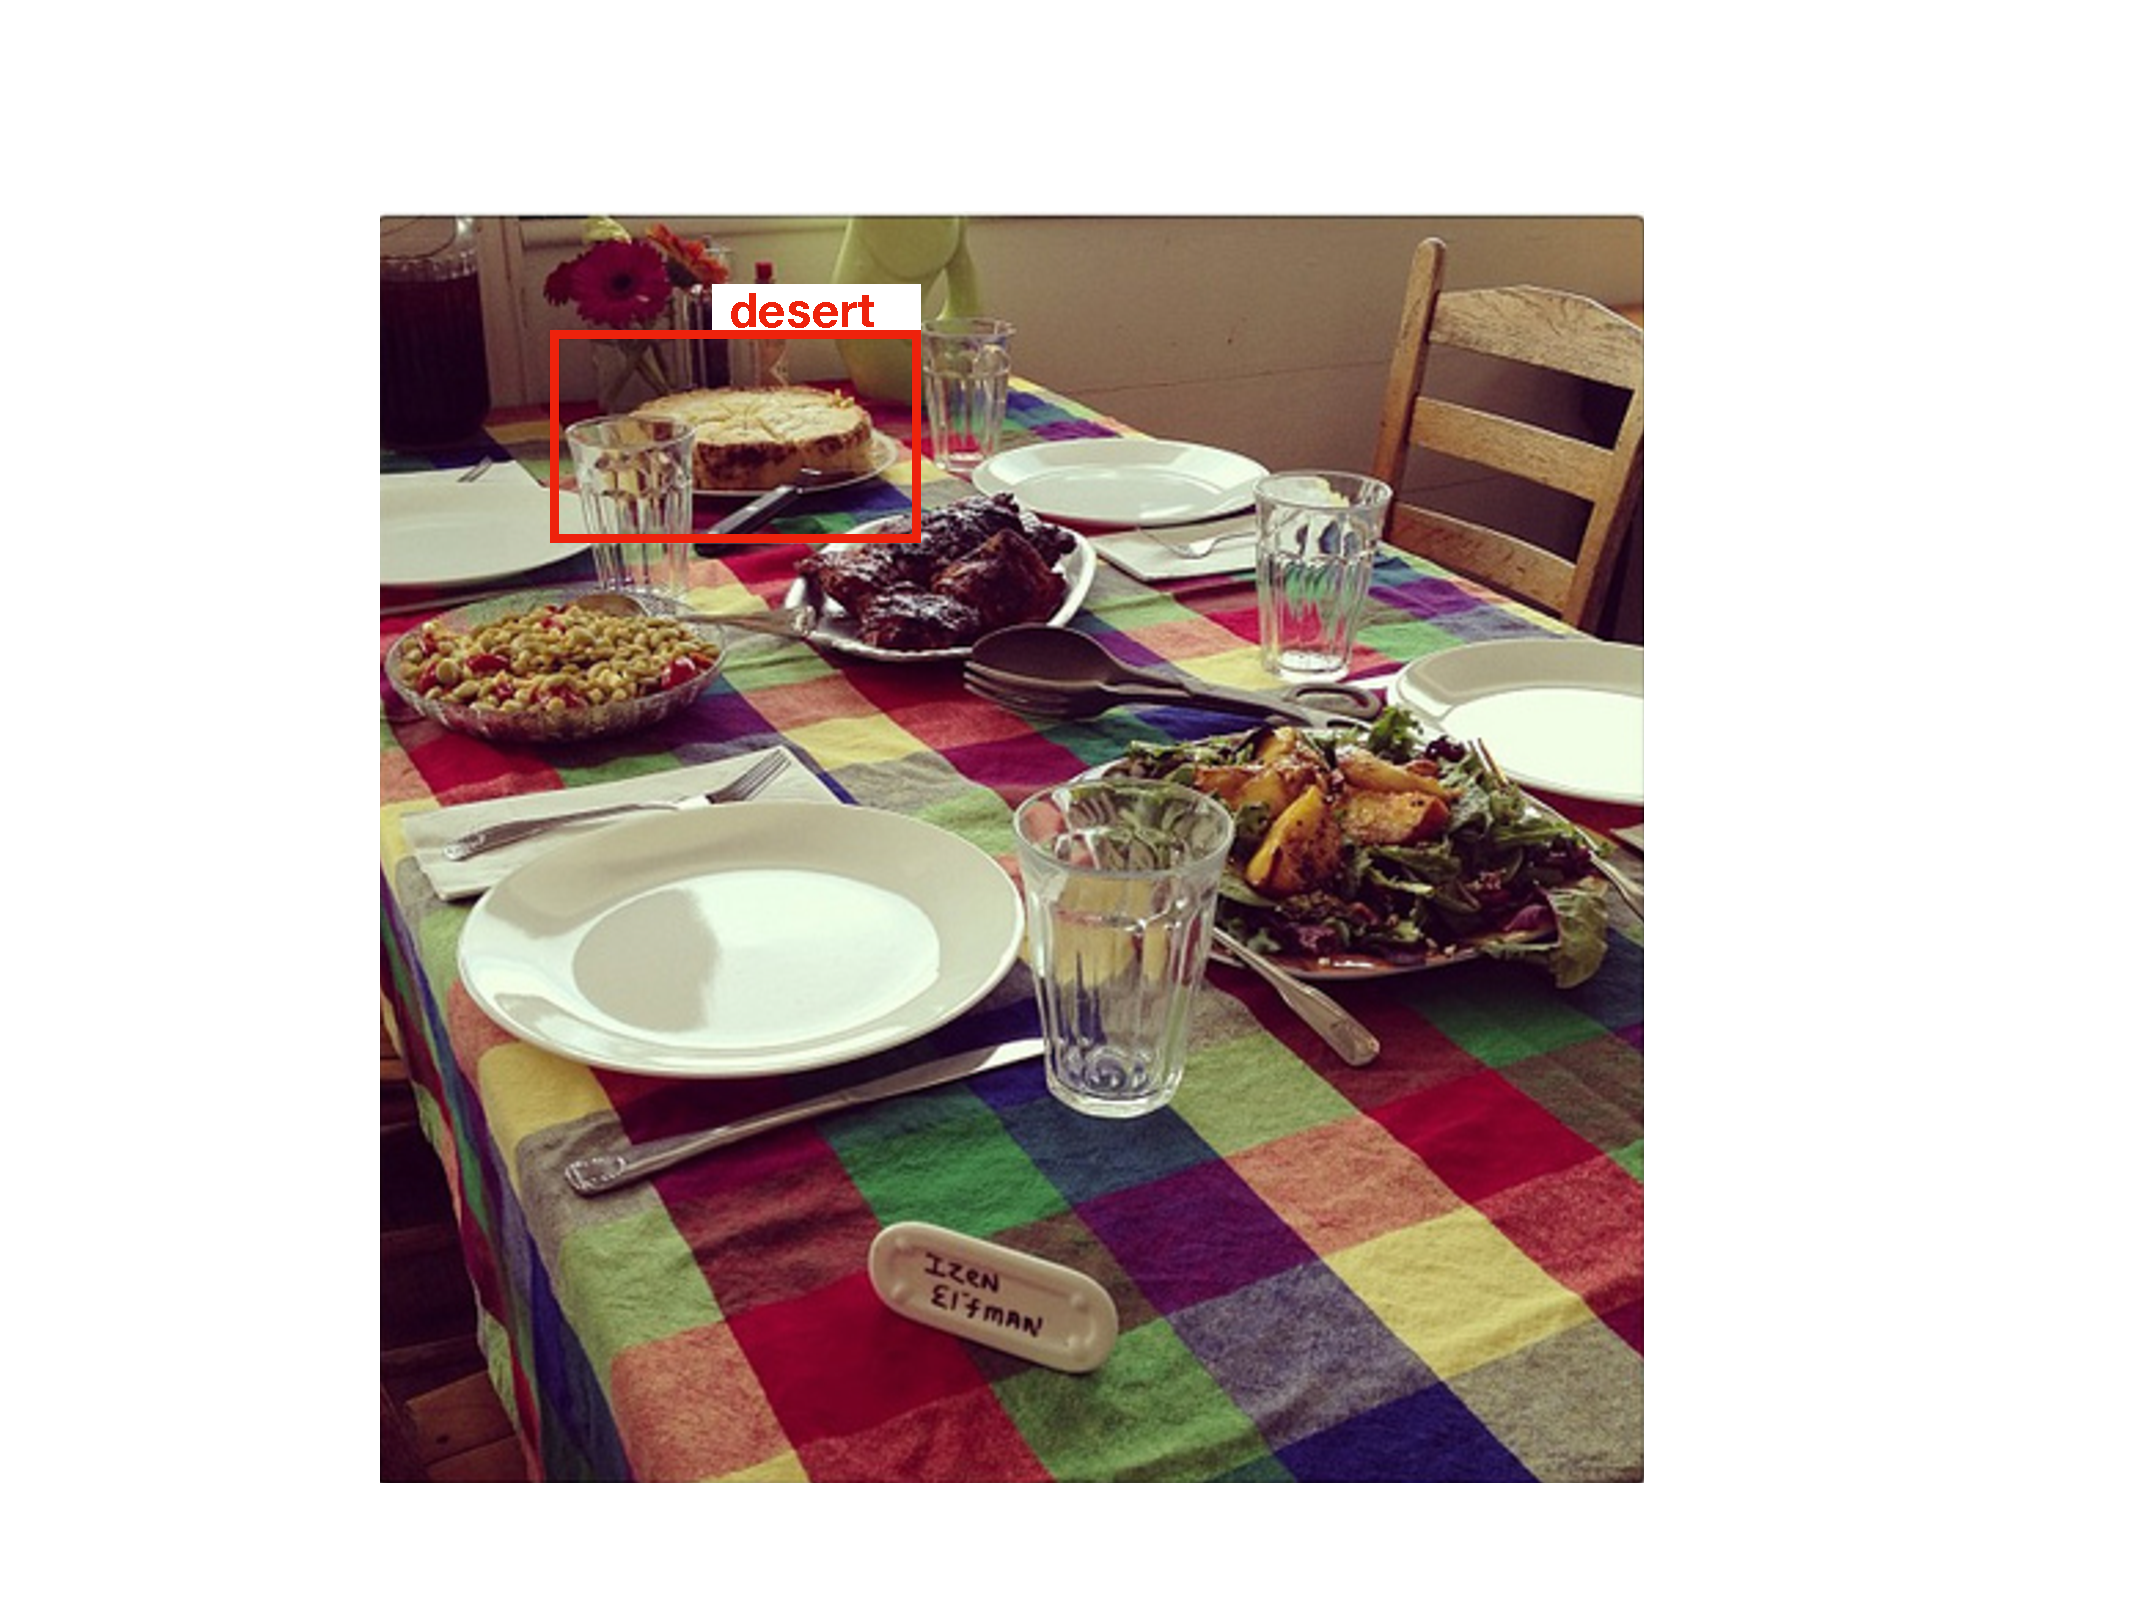
\includegraphics[height=3cm]{figures/cheesecak2.pdf}
\caption{Two objects of the same type of cake, with different names in VisualGenome}
\label{fig:cake}
\end{center}
\end{figure}

Our paper puts together two strands of research that have mostly been pursued independently to date.
On the one hand, state-of-the-art computer vision systems are able to accurately classify images into thousands of different categories (e.g.\  \newcite{googlenet}), where the task is often to predict the name for a given object. \gbt{Is this true? Imagenet task asks for synsets, which can be taken to be categories\dots To refine}
However, they mostly adopt very simple assumptions with respect to the underlying lexicon, which is implemented as a simple, flat labeling scheme: A standard object recognition system would be trained to classify the left object in Figure~\ref{fig:cake} as \emph{cheesecake}, the right one as \emph{dessert}, and using \emph{dessert} for the left picture would be considered incorrect.
On the other hand, research on object naming in Cognitive Science has shown that people choose different names depending on the circumstances, with factors such as context or the prototypicality of the object with respect to the category playing a role~\cite{add-refs}.
\gbt{This research also argues that there is high agreement in how people name objects; to do: make coherent.}
However, this research typically uses stylized drawings are used, and is focused on taxonomic relations (\textit{sparrow}-\textit{bird}).
\sz{It is thus unclear how findings from these stylized settings generalize to tasks in language \& vision like referring expression generation, where naming is a core aspect. Therefore, in contrast to traditional naming norm studies in Cognitive Science we study object naming in realistic scenes where objects are situated in a natural context! (This comes with additional challenges, like potential object occlusion, background/foreground confusion etc.)}

% Seminal work on prototypes suggests that the prototypicality of the object will determine the level of generality of the object name, i.e.\  a robin can be named \emph{bird}, but a penguin is better referred to as ``\emph{penguin}'' \cite{Rosch1978}.

% Two main findings in the literature:

% \begin{itemize}
% \item very high agreement, most people use the same name for the same object
% \item prototypicality is a factor, context too, but research has only looked at generality/specificity of the name
% \end{itemize}



In our study, we collect large-scale object naming data via crowdsourcing.
Like object naming studies in Cognitive Science, we collect multiple names per object (concretely, 36); like most work on language \& vision, we use natural images of common objects in context 
%\sz{(showing objects in complex visual contexts, surrounded by other objects, not ImageNet-like images)} 
on a large scale, annotating objects in 25K images from the VisualGenome dataset.
We analyze the agreement in object naming across subjects, and the sources of variation. We find that: \gbt{To be put in paragraph form}

\begin{itemize}
\item there is quite a high level of agreement in the task, with the relative frequency of the most common name being 70\% on average. This is in accordance with previous results in Cognitive Science~\cite{add-ref};
\item the level of agreement in object naming is much higher in certain domains than in others; as it happens, the domains that have been traditionally used in object naming research (e.g. animals) seem to display the highest amount of agreement in our data set;
\item most of the variation in our dataset comes from alternative names that do not stand in a taxonomic relation, suggesting that the previous work in Cognitive Science is missing much of the empirical ground.
%while previous work has mostly focused on variation in the level of generality within a taxonomy (\emph{penguin} vs. \emph{bird}), 

our datasets contains a lot of variability for names coming from different parts of the taxonomy (\emph{dessert} vs. \emph{cake}, \emph{bottle} vs. \emph{wine})
\end{itemize}

Moreover, we analyze whether current models implicitly encode the variation in naming, by doing XXX. We find YYY.


%The real-world objects that we interact with in our every-day life can be categorized into many thousands and maybe millions of categories. And even a single object can be member of many categories, i.e.\ at different taxonomical levels or in different parts of a taxonomy. For instance, both objects in Figure \ref{fig:cake} are at once instances of \cat{cake}, \cat{cheesecake}, \cat{dessert}, \cat{sweet}, \cat{pastry}, \cat{food} etc. Hence, when speakers name objects, e.g.\ when referring, they have to select a lexical item from a complex network of concepts and competing lexical alternatives.

%To date, research in NLP has surprisingly little to say about object naming, despite the fact that
% there has been a recent explosion of interest in various, and even complex, language \& vision tasks ranging from image captioning \cite{fangetal:2015,devlin:imcaqui,Bernardietal:automatic} to e.g.\ visual dialogue \cite{das2017visual,vries2017guesswhat}. 
%In contrast, closely related areas, such as computer vision and cognitive science, have investigated very related tasks in quite some depth: object recognition systems developed in the area of computer vision  are now able to classify images into thousands of different categories (e.g.\  \newcite{googlenet}).
%Furthermore, work on concepts, following the seminal work by Rosch, suggests that objects are typically conceptualized at a preferred level of specificity called the \textbf{entry-level}. Psycho-linguistic studies have been able to support this theory based on collections of so-called object naming norms. 
%
%This paper aims at addressing the genuinely linguistic questions revolving around the phenomenon of object naming by (i) presenting a collection of high-quality, large-scale naming data,  and (ii) analysis methods for this data and (iii) a first baseline model that accounts for the semantic flexibility of names for objects in real-world images. From computer vision, we borrow the idea of modeling realistic visual objects in realistic scenes (real-world images), but go beyond the simplistic assumption that object names correspond to unambiguous labels in a flat classification scheme (with no conceptual relations between the labels). From psycholinguistics, we borrow the idea of eliciting natural, representative naming data from many subjects, but go beyond using artificial, highly stylized objects.

%%% Local Variables:
%%% mode: latex
%%% TeX-master: "main"
%%% End:
